% Chapter 1

\chapter{Introducción General} % Main chapter title

\label{Chapter1} % For referencing the chapter elsewhere, use \ref{Chapter1} 
\label{IntroGeneral}

%----------------------------------------------------------------------------------------

% Define some commands to keep the formatting separated from the content 
\newcommand{\keyword}[1]{\textbf{#1}}
\newcommand{\tabhead}[1]{\textbf{#1}}
\newcommand{\code}[1]{\texttt{#1}}
\newcommand{\file}[1]{\texttt{\bfseries#1}}
\newcommand{\option}[1]{\texttt{\itshape#1}}
\newcommand{\grados}{$^{\circ}$}

%----------------------------------------------------------------------------------------

%\section{Introducción}

%----------------------------------------------------------------------------------------
\section{Aprendiendo \LaTeX{}}

\LaTeX{} no es \textsc{WYSIWYG} (What You See is What You Get), a diferencia de los procesadores de texto como Microsoft Word o Pages de Apple o incluso LibreOffice en el mundo open-source. En lugar de ello, un documento escrito para \LaTeX{} es en realidad un archivo de texto simple, llano que \emph{no contiene formato} . Nosotros le decimos a \LaTeX{} cómo deseamos que se aplique el formato en el documento final escribiendo comandos simples entre el texto, por ejemplo, si quiero usar \emph{texto en cursiva para dar énfasis}, escribo \verb|\emph{texto}| y pongo el texto en cursiva que quiero entre medio de las llaves. Esto significa que \LaTeX{} es un lenguaje del tipo \enquote{mark-up}, muy parecido a HTML.

\subsection{Una introducción (no tan corta) a \LaTeX{}}

Si usted es nuevo a \LaTeX{}, hay un muy buen libro electrónico - disponible gratuitamente en Internet como un archivo PDF - llamado, \enquote{A (not so short) Introduction to \LaTeX{}}. El título del libro es generalmente acortado a simplemente \emph{lshort}. Puede descargar la versión más reciente en inglés (ya que se actualiza de vez en cuando) desde aquí:
\url{http://www.ctan.org/tex-archive/info/lshort/english/lshort.pdf}

Está disponible en varios idiomas además del inglés. Se puede encontrar la versión en español en la lista en esta página: \url{http://www.ctan.org/tex-archive/info/lshort/}


\subsection{Guía matemática rápida para \LaTeX{}}

Si usted está escribiendo un documento con mucho contenido matemático, entonces es posible que desee leer el documento de la AMS (American Mathematical Society) llamado, \enquote{A Short Math Guide for \LaTeX{}}. Se puede encontrar en línea en el siguiente link: \url{http://www.ams.org/tex/amslatex.html} en la sección \enquote{Additional Documentation} hacia la parte inferior de la página.


%----------------------------------------------------------------------------------------

\section{Utilizando esta plantilla}

Si usted está familiarizado con \LaTeX{}, entonces puede explorar la estructura de directorios de esta plantilla y proceder a personalizarla agregando su información en el bloque \emph{INFORMACIÓN DE LA PORTADA} en el archivo \file{memoria.tex}.  

Se puede continuar luego modificando el resto de los archivos siguiendo los lineamientos que se describen en la sección \ref{sec:FillingFile} en la página \pageref{sec:FillingFile}.

Asegúrese de leer el capítulo \ref{Chapter2} acerca de las convenciones utilizadas para las Memoria de los Trabajos Finales de la Carrera de Especialización en Sistemas Embebidos de FIUBA.

Si es nuevo en \LaTeX{} se recomienda que continue leyendo el documento ya que contiene información básica para aprovechar el potencial de esta herramienta.


\subsection{Acerca de esta plantilla}

Esta plantilla \LaTeX{} está basada originalmente en torno a un archivo de estilo \LaTeX{} creado por Steve R.\ Gunn de la  University of Southampton (UK), department of Electronics and Computer Science. Se puede encontrar su trabajo original en el siguiente sitio de internet:
\url{http://www.ecs.soton.ac.uk/~srg/softwaretools/document/templates/}

El archivo de Gunn, \file{ecsthesis.cls} fue posteriormente modificado por Sunil Patel quien creó una plantilla esqueleto con la estructura de carpetas. El template resultante se puede encontrar en el sitio web de Sunil Patel:
\url{http://www.sunilpatel.co.uk/thesis-template}

El template de Patel se publicó a través de  \url{http://www.LaTeXTemplates.com} desde donde fue modificado muchas veces en base a solicitudes de usuarios. La versión 2.0 y subsiguientes representan cambios significativos respecto a la versión de la plantilla modificada por Patel, que es de hecho, dificilmente reconocible. El trabajo en la version 2.0 fue realizado por Vel Gayevskiy y Johannes Böttcher.

Para la Carrera de Especialización en Sistemas Embebidos de FIUBA, la versión versión 2.3 fue modificada por el Ing. \href{mailto:pbos@fi.uba.ar}{Patricio Bos} para crear una plantilla fuertemente adaptada a la carrera de especialización.

%----------------------------------------------------------------------------------------

\section{Qué incluye esta plantilla}

\subsection{Carpetas}

Esta plantilla se distribuye como una único archivo .zip que se puede descomprimir en varios archivos y carpetas. Los nombres de las carpetas son (o pretender ser) auto-explicativos.

\keyword{Appendices} -- Esta es la carpeta donde se deben poner los apéndices. Cada apéndice debe ir en su propio archivo \file{.tex}. Se incluye un ejemplo y una plantilla en la carpeta.

\keyword{Chapters} -- Esta es la carpeta donde se deben poner los capítulos de la memoria. Cada capítulo debe ir un su propio archivo \file{.tex} por separado.  Se ofrece por defecto, la siguiente estructura de capítulos y se recomienda su utilización dentro de lo posible:

\begin{itemize}
\item Capítulo 1: Introducción general	
\item Capítulo 2: Introducción específica
\item Capítulo 3: Diseño e implementación
\item Capítulo 4: Ensayos y resultados
\item Capítulo 5: Conclusiones

\end{itemize}

Esta estructura de capítulos es la que se recomienda para las memorias de la especialización.

\keyword{Figures} -- Esta carpeta contiene todas las figuras de la memoria.  Estas son las versiones finales de las imágenes que van a ser incluidas en la memoria.  Pueden ser imágenes en formato \textit{raster}\footnote{\url{https://en.wikipedia.org/wiki/Raster_graphics}} como \file{.png}, \file{.jpg} o en formato vectoriales\footnote{\url{https://en.wikipedia.org/wiki/Vector_graphics}} como \file{.pdf}, \file{.ps}.  Se debe notar que utilizar imágenes vectoriales disminuye notablemente el peso del documento final y acelera el tiempo de compilación por lo que es recomendable su utilización siempre que sea posible.

\subsection{Archivos}

También están incluidos varios archivos, la mayoría de ellos son de texto plano y se puede ver su contenido en un editor de texto. Después de la compilación inicial, se verá que más archivos auxiliares son creados por \ LaTeX{} o BibTeX, pero son de uso interno y que no es necesario eliminarlos o hacer nada con ellos.  Toda la información necesaria para complilar el documento se encuentra en los archivos \file{.tex} y en las imágenes de la carpeta Figures.

\keyword{referencias.bib} - este es un archivo importante que contiene toda la información de referencias bibliográficas que se utilizarán para las citas en la memoria en conjunto con BibTeX. Usted puede escribir las entradas bibliográficas en forma manual, aunque existen también programas de gestión de referencias que facilitan la creación y gestión de las referencias y permiten exportarlas en formato BibTeX.  También hay disponibles sitios web como \url{books.google.com} que permiten obtener toda la información necesaria para una cita en formato BibTeX. Ver sección \ref{sec:biblio}

\keyword{MastersDoctoralThesis.cls} -- este es un archivo importante. Es el archivos con la clase que le informa a \LaTeX{} cómo debe dar formato a la memoria. El usuario de la plantilla no debería necesitar modificar nada de este archivo.

\keyword{memoria.pdf} -- esta es su memoria con una tipografía bellamente compuesta (en formato de archivo PDF) creado por \LaTeX{}. Se distribuye con la plantilla y después de compilar por primera vez sin hacer ningún cambio se debería obtener una versión idéntica a este documento.

\keyword{memoria.tex} -- este es un archivo importante. Este es el archivo que tiene que compilar \LaTeX{} para producir la memoria como un archivo PDF. Contiene un marco de trabajo y estructuras que le indican a \LaTeX{} cómo diagramar la memoria.  Está altamente comentado para que se pueda entender qué es lo que realiza cada línea de código y por qué está incluida en ese lugar.  En este archivo se debe completar la información personalizada de las primeras sección según se indica en la sección \ref{sec:FillingFile}.

Archivos que \emph{no} forman parte de la distribución de la plantilla pero que son generados por \LaTeX{} como archivos auxiliares necesarios para la producción de la memoria.pdf son:

\keyword{memoria.aux} -- este es un archivo auxiliar generado por \LaTeX{}, si se borra \LaTeX{} simplemente lo regenera cuando se compila el archivo principal \file{memoria.tex}.

\keyword{memoria.bbl} -- este es un archivo auxiliar generado por BibTeX, si se borra BibTeX simplemente lo regenera cuando se compila el archivo principal \file{memoria.tex}. Mientras que el archivo \file{.bib} contiene todas las referencias que hay, este archivo \file{.bbl} contine sólo las referencias que han sido citadas y se utiliza para la construcción de la bibiografía.

\keyword{memoria.blg} -- este es un archivo auxiliar generado por BibTeX, si se borra BibTeX simplemente lo regenera cuando se compila el archivo principal \file{memoria.tex}.

\keyword{memoria.lof} -- este es un archivo auxiliar generado por \LaTeX{}, si se borra \LaTeX{} simplemente lo regenera cuando se compila el archivo principal \file{memoria.tex}.  Le indica a \LaTeX{} cómo construir la sección \emph{Lista de Figuras}.
 
\keyword{memoria.log} --  este es un archivo auxiliar generado por \LaTeX{}, si se borra \LaTeX{} simplemente lo regenera cuando se compila el archivo principal \file{memoria.tex}. Contiene mensajes de \LaTeX{}. Si se reciben errores o advertencias durante la compilación, se guardan en este archivo \file{.log}.

\keyword{memoria.lot} -- este es un archivo auxiliar generado por \LaTeX{}, si se borra \LaTeX{} simplemente lo regenera cuando se compila el archivo principal \file{memoria.tex}.  Le indica a \LaTeX{} cómo construir la sección \emph{Lista de Tablas}.

\keyword{memoria.out} -- este es un archivo auxiliar generado por \LaTeX{}, si se borra \LaTeX{} simplemente lo regenera cuando se compila el archivo principal \file{memoria.tex}.

De esta larga lista de archivos, sólo aquellos con la extensión \file{.bib}, \file{.cls} y \file{.tex} son importantes.  Los otros archivos auxiliares pueden ser ignorados o borrados ya que \LaTeX{} y BibTeX los regenerarán durante la compilación.

%----------------------------------------------------------------------------------------

\section{Entorno de trabajo}

Ante de comenzar a editar la plantilla debemos tener un editor \LaTeX{} instalado en nuestra computadora.  En forma análoga a lo que sucede en lenguaje C, que se puede crear y editar código con casi cualquier editor, exiten ciertos entornos de trabajo que nos pueden simplificar mucho la tarea.  En este sentido, se recomienda, sobre todo para los principiantes en \LaTeX{} la utilización de TexMaker, un programa gratuito y multi-plantaforma que está disponible tanto para windows como para sistemas GNU/linux.

La versión más reciente de TexMaker es la 4.5 y se puede descargar del siguiente link: \url{http://www.xm1math.net/texmaker/download.html}. Se puede consultar el manual de usuario en el siguiente link: \url{http://www.xm1math.net/texmaker/doc.html}.
 

\subsection{Paquetes adicionales}

Si bien durante el proceso de instalación de TexMaker, o cualquier otro editor que se haya elegido, se instalarán en el sistema los paquetes básicos necesarios para trabajar con \LaTeX{}, la plantilla de los trabajos de Especialización y Maestría requieren de paquete adicionales.

Se indican a continuación los comandos que se deben introducir en la consola de Ubuntu (ctrl + alt + t) para instalarlos:

\begin{lstlisting}[language=bash]
  $ sudo apt install texlive-lang-spanish texlive-science 
  $ sudo apt install texlive-bibtex-extra biber
  $ sudo apt install texlive texlive-fonts-recommended
\end{lstlisting}


\subsection{Configurando TexMaker}


Una vez instalado el programa y los paquetes adicionales se debe abrir el archivo memoria.tex con el editor para ver una pantalla similar a la que se puede apreciar en la figura \ref{fig:texmaker}. 

\begin{figure}[h]
	\centering
	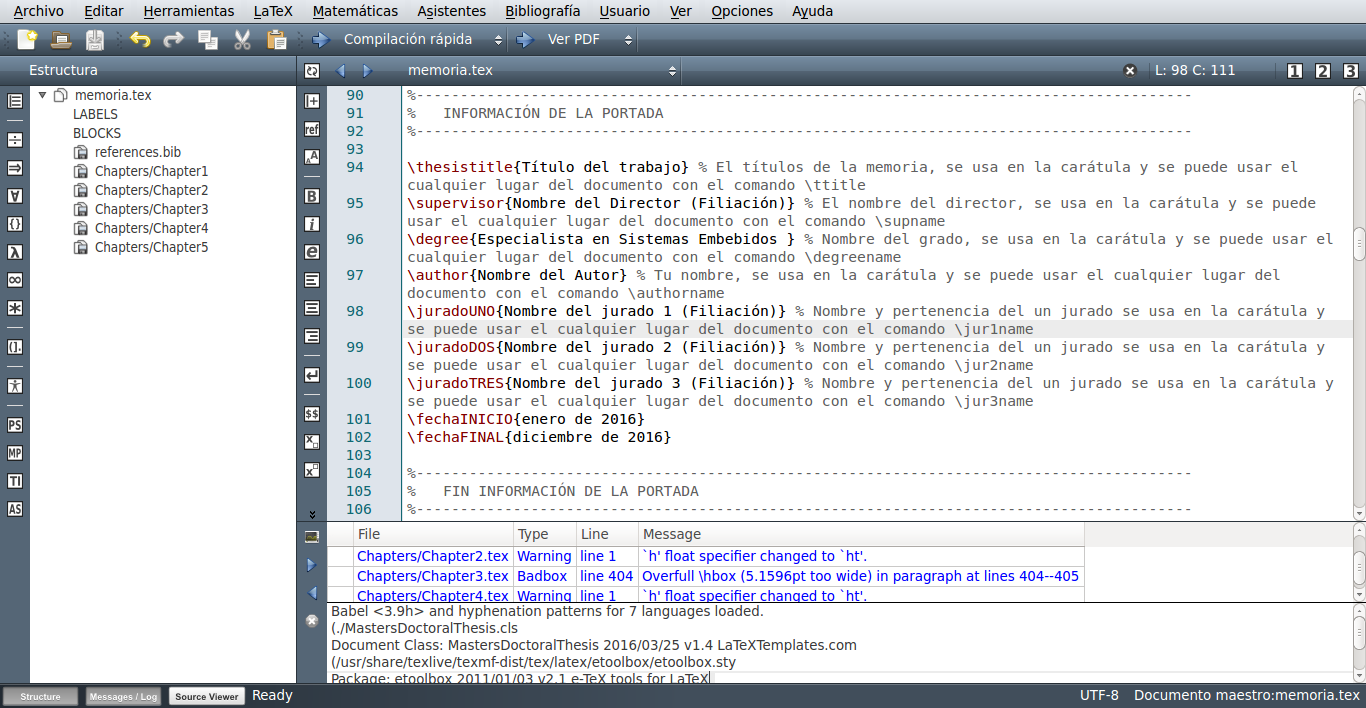
\includegraphics[width=\textwidth]{./Figures/texmaker.png}
	\caption{Entorno de trabajo de texMaker.}
	\label{fig:texmaker}
\end{figure}

Notar que existe una vista llamada Estructura a la izquierda de la interface que nos permite abrir desde dentro del programa los archivos individuales de los capítulos.  A la derecha se encuentra una vista con el archivo propiamente dicho para su edición. Hacia la parte inferior se encuentra una vista del log con información de los resultados de la compilación.  En esta última vista pueden aparecen advertencias o \textit{warning}, que normalmente pueden ser ignorados, y los errores que se indican en color rojo y deben resolverse para que se genere el PDF de salida.

Recordar que el archivo que se debe compilar con PDFLaTeX es \file{memoria.tex}, si se tratara de compilar alguno de los capítulos saldría un error.  Para salvar la molestia de tener que cambiar de archivo para compilar cada vez que se realice una modificación en un capítulo, se puede definir el archivo \file{memoria.tex} como ``documento maestro'' yendo al menú opciones -> ``definir documento actual como documento maestro'', lo que permite compilar con PDFLaTeX memoria.tex directamente desde cualquier archivo que se esté modificando . Se muestra esta opción en la figura \ref{fig:docMaestro}.

\begin{figure}[h]
	\centering
	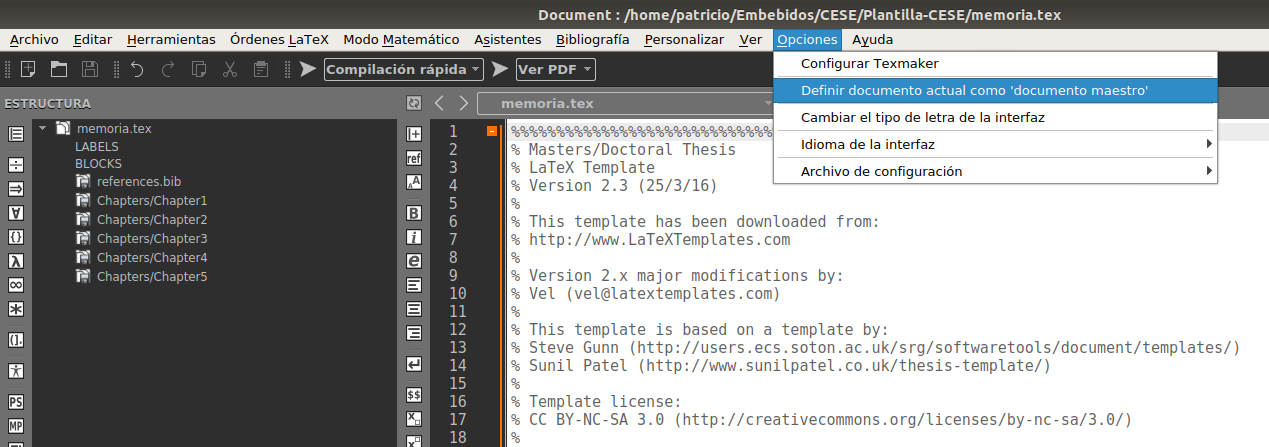
\includegraphics[width=\textwidth]{./Figures/docMaestro.png}
	\caption{Definir memoria.tex como documento maestro.}
	\label{fig:docMaestro}
\end{figure}

En el menú herramientas se encuentran las opciones de compilación.  Para producir un archivo PDF a partir de un archivo .tex se debe ejecutar PDFLaTeX (el shortcut es F6). Para incorporar nueva bibliografía se debe utilizar la opción BibTeX del mismo menú herramientas (el shortcut es F11).

Notar que para actualizar las tablas de contenidos se debe ejecutar PDFLaTeX dos veces.  Esto se debe a que es necesario actualizar algunos archivos auxiliares antes de obtener el resultado final.  En forma similar, para actualizar las referecias se debe ejecutar primero PDFLaTeX, después BibTeX y finalmente PDFLaTeX dos veces por idénticos motivos.

\section{Personalizando la plantilla, el archivo \file{memoria.tex}}
\label{sec:FillingFile}

Para personalizar la plantilla se debe incorporar la información propia en los distintos archivos \file{.tex}. 

Primero abrir \file{memoria.tex} con TexMaker (o el editor de su preferencia). Se debe ubicar dentro del archivo el bloque de código titulado \emph{INFORMACIÓN DE LA PORTADA} donde se deben incorporar los primeros datos personales con los que se constuirá automáticamente la portada.


%----------------------------------------------------------------------------------------

\section{El código del archivo \file{memoria.tex} explicado}

El archivo \file{memoria.tex} contiene la estructura del documento y es el archivo de mayor jeraquía de la memoria.  Podría ser equiparable a la función \emph{main()} de un programa en C, o mejor dicho al archivo fuente .c donde se encuentra definida la función main().

La estructura básica de cualquier documento de \LaTeX{} comienza con la definición de clase del documento, es seguida por un preámbulo donde se pueden agregar funcionalidades con el uso de \texttt{paquetes} (equiparables a bibliotecas de C), y finalmente, termina con el cuerpo del documento, donde irá el contenido de la memoria.

\lstset{%
  basicstyle=\small\ttfamily,
  language=[LaTeX]{TeX}
}

\begin{lstlisting}
\documentclass{article}  <- Definicion de clase
\usepackage{listings}	 <- Preambulo

\begin{document}	 <- Comienzo del contenido propio 
	Hello world!
\end{document}
\end{lstlisting}


El archivo \file{memoria.tex} se encuentra densamente comentado para explicar qué páginas, secciones y elementos de formato está creando el código \LaTeX{} en cada línea. El código está dividido en bloques con nombres en mayúsculas para que resulte evidente qué es lo que hace esa porción de código en particular. Inicialmente puede parecer que hay mucho código \LaTeX{}, pero es principalmente código para dar formato a la memoria por lo que no requiere intervención del usuario de la plantilla.  Sí se deben personalizar con su información los bloques indicados como:

\begin{itemize}
	\item Informacion de la memoria
	\item Carátula
	\item Resumen
	\item Agradecimientos
	\item Dedicatoria
\end{itemize}

El índice de contenidos, las listas de figura de tablas se generan en forma automática y no requieren intervención ni edición manual por parte del usuario de la plantilla. 

En la parte final del documento se encuentran los capítulos y los apéndices.  Por defecto se incluyen los 5 capítulos propuestos que se encuentran en la carpeta /Chapters. Cada capítulo se debe escribir en un archivo .tex separado y se debe poner en la carpeta \emph{Chapters} con el nombre \file{Chapter1}, \file{Chapter2}, etc\ldots El código para incluir capítulos desde archivos externos se muestra a continuación.

\begin{verbatim}
	% Chapter 1

\chapter{Introducción General} % Main chapter title

\label{Chapter1} % For referencing the chapter elsewhere, use \ref{Chapter1} 
\label{IntroGeneral}

%----------------------------------------------------------------------------------------

% Define some commands to keep the formatting separated from the content 
\newcommand{\keyword}[1]{\textbf{#1}}
\newcommand{\tabhead}[1]{\textbf{#1}}
\newcommand{\code}[1]{\texttt{#1}}
\newcommand{\file}[1]{\texttt{\bfseries#1}}
\newcommand{\option}[1]{\texttt{\itshape#1}}
\newcommand{\grados}{$^{\circ}$}

%----------------------------------------------------------------------------------------

%\section{Introducción}

%----------------------------------------------------------------------------------------

En este capítulo se realiza una introducción al concepto de Internet de las Cosas, se describe la motivación del trabajo realizado y se presentan sus objetivos y alcance.

\section{Internet de las Cosas{}}

Desde la aparición de Internet a finales del siglo pasado, ha quedado demostrado lo útil que es contar con un dispositivo capaz de conectarse a la red. Los beneficios de que una computadora o un teléfono inteligente puedan conectarse a Internet son evidentes, y esos beneficios también se encuentran presentes al conectar cualquier otro objeto a Internet, y es allí donde surge el concepto de Internet de las Cosas (IoT, por sus siglas en inglés correspondientes a \emph{Internet of Things}).

La Internet de las Cosas consiste en extender el potencial de Internet y la conectividad más allá de las computadoras y celulares, e incorporar a todos los objetos (cosas) de la vida cotidiana y que se encuentran presentes en el entorno de una persona. Así se permite tanto la comunicación e interacción entre sí de estos objetos, como así también el monitoreo y control en forma remota.

El concepto de \enquote{cosa} es sumamente amplio, ya que contempla desde lámparas, cerraduras y termostatos en el hogar, hasta maquinaria industrial y sistemas de riego para agricultura, pasando por vehículos autónomos, sistemas de iluminación y sensores para estacionamiento público en una ciudad. El objeto conectado incluso puede ser un monitor cardíaco en el interior de una persona o un chip insertado en un animal de granja. Gracias a la existencia de sensores y microcontroladores cada vez más potentes, más pequeños y de menor costo, es posible lograr que prácticamente cualquier dispositivo forme parte del ecosistema IoT.

Los beneficios que la Internet de las Cosas ofrece tanto a empresas como a personas individuales son innumerables. Desde un punto de vista económico, les da la posibilidad a las empresas de conocer y monitorear mejor sus procesos, para así hacerlos más eficientes y posibilitar mejores tomas de decisiones y acciones como mantenimiento predictivo de maquinaria. Todo eso se traduce en definitiva en un ahorro de dinero y tiempo para la organización. Con respecto a un individuo particular, la Internet de las Cosas le permite mejorar su calidad de vida y su comodidad en el día a día con automatizaciones en el hogar (domótica), como así también beneficios a la salud con, por ejemplo, implantes inteligentes que permiten un cuidadoso monitoreo.

Las empresas, las personas y el mercado en general hace ya varios años que se han dado cuenta de la importancia de la Internet de las Cosas. Es prueba de ello la gran cantidad de dispositivos conectados que existen, y las proyecciones que indican que estos números seguirán aumentando notablemente. En 2017 ya había 27 mil millones de dispositivos IoT conectados, cifra que aumentará a un ritmo de un 12\% anual hasta llegar a 125 mil millones para 2030 \citep{1}. Por otra parte, en la figura \ref{fig:iot_market} se puede observar cómo el mercado mundial de la Internet de las Cosas ya maneja cantidades de dinero superiores a los USD 200.000.000.000, y cómo esa cifra aumentará sustancialmente a lo largo de los próximos años \citep{2}, lo cual supone una enorme oportunidad de negocio para muchas empresas.

\begin{figure}[h]
\centering
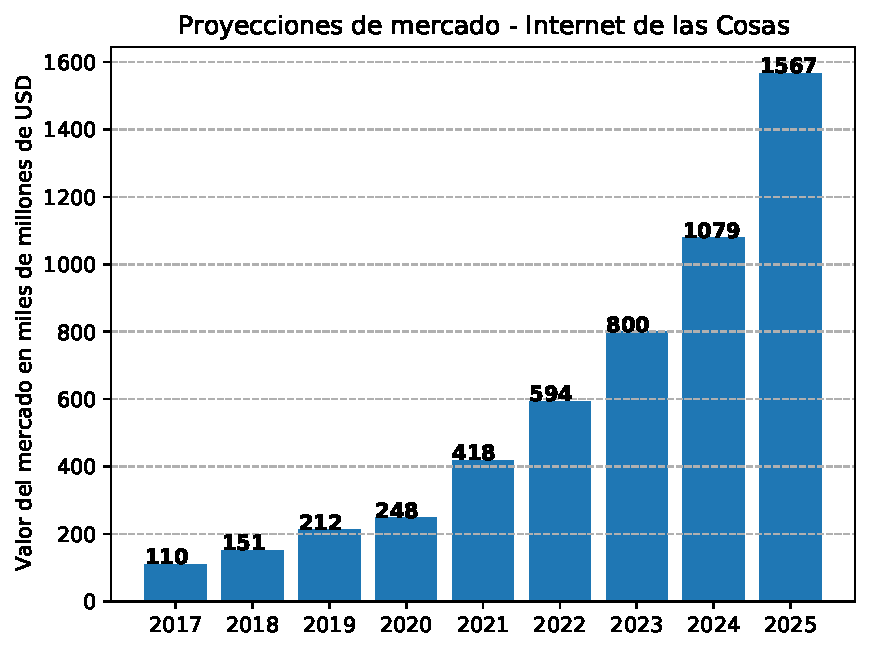
\includegraphics[width=\textwidth]{./Figures/iot_market_projection.pdf}
\caption[Proyecciones del valor de mercado a nivel mundial de la Internet de las Cosas.]{Proyecciones del valor de mercado a nivel mundial de la Internet de las Cosas.\footnotemark}
\label{fig:iot_market}
\end{figure}

\footnotetext{Gráfico replicado en base al que se muestra en \url{https://www.statista.com/statistics/976313/global-iot-market-size/}.}


Por último, un punto que a menudo es pasado por alto al momento de hablar de la Internet de las Cosas, son todos los problemas asociados a la seguridad y la privacidad. Tener un mayor número de dispositivos conectados, muchos de los cuales recolectan información sumamente sensible, expande la superficie de ataque considerablemente, y deja tanto a empresas como a personas más vulnerables frente a posibles \emph{hackers}. Existen incontables ejemplos de vulnerabilidades en dispositivos IoT que salieron a la luz, como una gigantesca \emph{botnet} formada por dispositivos IoT \citep{3}, televisores inteligentes que espían conversaciones privadas \citep{4}, e incluso ataques dirigidos a dispositivos conectados en entornos industriales \citep{5}. Estos hechos ocurren principalmente porque la seguridad y la privacidad a menudo son vistas como costos extra en los que no vale la pena incurrir. Incluso en ocasiones la propia empresa utiliza de manera poco ética esos agujeros de seguridad para obtener datos de los usuarios y sacar algún tipo de provecho económico a partir de ellos.

Las consecuencias de una falla de seguridad en un dispositivo IoT pueden ser muy graves, por lo que al momento de desarrollar una solución en el segmento del Internet de las Cosas, los aspectos de seguridad deben ser tenidos en consideración desde un principio, aún cuando ello implique desarrollar un producto más costoso o complejo.

\section{Estado del arte{}}
\label{sec:estado_del_arte}

En la actualidad, existe una enorme cantidad de dispositivos conectados que pertenecen a muy diversos ámbitos, por lo que resultaría poco práctico brindar un panorama general del estado del arte en todos ellos. Por lo tanto, el foco estará en aquellos productos que ofrezcan soluciones orientadas a dispositivos que ya cuentan con cierto nivel de ''inteligencia'' (como maquinaria industrial/agrícola o artefactos del hogar), a los fines de dotarlos de conectividad y de todo un entorno que permita procesar y analizar los datos generados por ellos.

Por un lado, existen numerosas plataformas que solamente ofrecen la etapa de procesamiento, análisis y visualización de datos. Estas plataformas asumen que el cliente cuenta con el hardware necesario para enviarles la información relevante, y ellas se encargan de analizarla y presentarla de manera conveniente mediante tableros o \emph{dashboards}, que le permiten al usuario ver el estado de los dispositivos y actuar sobre ellos. La mayoría de estas plataformas poseen características similares tales como administración de dispositivos, visualización de datos y soporte a múltiples protocolos de comunicación. Algunos ejemplos de esta clase de plataformas son ThingBoard \citep{7}, Thinger \citep{8} y Ubidots \citep{9}, además de los servicios específicamente orientados a IoT de Amazon Web Services, de Google Cloud Platform y de Microsoft Azure.  

Por otra parte, existen también plataformas de hardware que ofrecen soluciones genéricas de conectividad, junto con plataformas para analizar y visualizar los datos obtenidos, con características similares a las mencionadas anteriormente.

En este último segmento hay diferentes grados de especialización. Por ejemplo, existen empresas que ofrecen soluciones orientadas exclusivamente al ámbito industrial, como ThingWorx de la empresa PTC \citep{10}, mientras que otras brindan soluciones más genéricas con una plataforma de hardware y un entorno de análisis y visualización, como el caso de Particle (figura \ref{fig:particle_iot}) \citep{11}.

\begin{figure}[h]
\centering
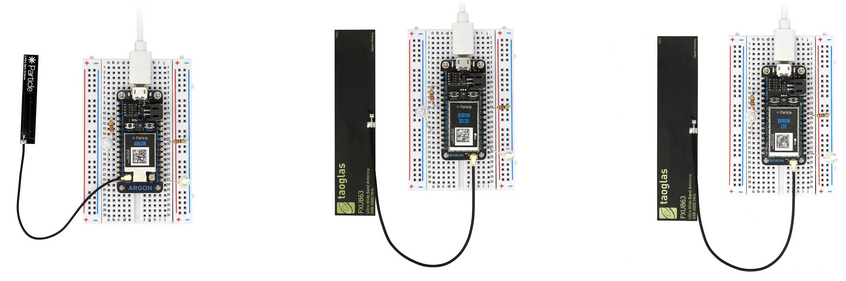
\includegraphics[scale=0.4]{./Figures/particle_iot.png}
\caption[Plataformas de hardware ofrecidas por Particle.]{Plataformas de hardware ofrecidas por Particle.\footnotemark}
\label{fig:particle_iot}
\end{figure}

\footnotetext{Imagen extraída de \url{https://store.particle.io/pages/prototyping-hardware}.}


\section{Motivación{}}

Un sector fundamental en el ámbito del Internet de las Cosas es el de la domótica, es decir el conjunto de tecnologías que permite el control y la automatización inteligente de una vivienda, a los fines de lograr una gestión eficiente y brindar mayor comodidad y seguridad a quienes la habitan \citep{6}.

A su vez, dentro de la domótica, un campo de especial interés es el de los electrodomésticos inteligentes (o \emph{smart appliances}), tales como televisores, heladeras, hornos, lavarropas o microondas. 

Una característica primordial de un electrodoméstico inteligente es su capacidad de
estar conectado y ser manejado o accedido de forma remota, ya sea mediante una plataforma web, una aplicación en el celular, comandos de voz o cualquier otro medio. Esta capacidad brinda grandes ventajas con respecto a un artefacto convencional, ya que no solamente ofrece una mayor comodidad al momento de usarlo, sino que también permite programar acciones (como preparar un café a una determinada hora) y ahorrar energía al hacer más eficiente su uso.

Actualmente existen ya en el mercado numerosos ejemplos de electrodomésticos inteligentes que permiten llevar a cabo diferentes acciones:
\begin{itemize}
	\item Encender el horno mediante un comando de voz, incluso con integración con los asistentes de voz más comunes.
	\item Consultar el contenido de la heladera mediante una aplicación en el celular.
	\item Recibir una notificación cuando el ciclo de lavado del lavarropas finaliza.
	\item Diagnosticar automáticamente la causa de una falla.
\end{itemize}

Gracias a las ventajas que ofrecen, la demanda de electrodomésticos inteligentes es cada vez más mayor, por lo que aquellas empresas o fabricantes que no se modernicen y comiencen a incorporar características \emph{smart} a sus dispositivos, se encontrarán en clara desventaja
al competir en el mercado con aquellas que sí lo hagan.

Como se puede apreciar en la sección \ref{sec:estado_del_arte}, existen ya en el mercado numerosas soluciones orientadas a la Internet de las Cosas. Cada una de ellas ofrece diferentes características y cubre diferentes mercados. Dentro de las soluciones que ofrecen una plataforma tanto de hardware como de software, no existe un sector consolidado que esté orientado a dotar de conectividad a electrodomésticos en el hogar, y es allí donde surge la importancia del presente trabajo. Lo que se busca es cubrir justamente ese sector y ofrecer una solución personalizada a los fabricantes para que puedan lograr que los electrodomésticos que ya fabrican se conviertan en electrodomésticos inteligentes.


\section{Objetivos y alcance{}}

\subsection{Objetivos generales}

El objetivo general del presente trabajo es el diseño e implementación de un módulo capaz de dotar de conectividad WiFi y Bluetooth a un electrodoméstico convencional. Para ello, el módulo debe tener la capacidad de comunicarse con la placa del propio equipo y de recibir/enviar información a un servidor en la nube, a los fines de permitirle al usuario final un manejo remoto del aparato y conocer su estado, como así también enviar información de uso al fabricante. 

El módulo no está destinado directamente al usuario final del electrodoméstico, sino a empresas o fabricantes que busquen incorporar características inteligentes a sus electrodomésticos.

A grandes rasgos, desde el punto de vista del usuario final, se debe permitir:
\begin{itemize}
	\item Enviar por WiFi o Bluetooth un comando al electrodoméstico que dispare una acción en él, como iniciar la cocción en un horno o el lavado en un lavarropas.
	\item Conocer el estado del electrodoméstico mediante la recepción de información por WiFi o Bluetooth.
\end{itemize}

Por otra parte, desde el punto de vista del fabricante del electrodoméstico se debe permitir:
\begin{itemize}
	\item Recibir y almacenar información acerca del estado de todos los dispositivos (si están o o no conectados, y en qué estado de ejecución se encuentran).
	\item Analizar y visualizar de manera conveniente la información de estado de los dispositivos a lo largo del tiempo.
\end{itemize}

\subsection{Alcance}

El presente trabajo incluye los siguientes aspectos:

\begin{enumerate}
	\item Análisis, investigación y elección del hardware a utilizar en el módulo.
	\item Implementación del firmware del sistema.
	\item Comunicación con un microcontrolador que emule el comportamiento del electrodoméstico.
	\item Desarrollo de una interfaz web mediante una plataforma ya existente, que permita enviarle comandos al electrodoméstico emulado.
	\item Implementación de un entorno en la nube que permita analizar y visualizar los datos de los diferentes electrodomésticos conectados.
\end{enumerate}

Es de especial importancia el punto 3 de la lista, en el que se define explícitamente que, a los fines de agilizar considerablemente el tiempo de desarrollo del trabajo, el prototipo no se utilizará en un electrodoméstico real. La interacción con él se emula mediante la comunicación con otro microcontrolador, que actúa como la placa de control del electrodoméstico: imita su comportamiento y sus respuestas ante diferentes estímulos.

En línea con el párrafo anterior, el presente trabajo no incluye lo siguiente:

\begin{enumerate}
	\item Integración del prototipo a diferentes electrodomésticos/marcas con distintos tipos de
comunicación serie y funcionalidades.
	\item Desarrollo de una aplicación móvil desde la cual interactuar por Bluetooth con el módulo.
	\item Diseño y fabricación de un circuito impreso. Para el trabajo se utiliza una placa de prototipo ya existente que incluye el hardware seleccionado.
\end{enumerate}






















 
	\chapter{Introducción Específica}
\label{Chapter2}

En el presente capítulo se brinda una explicación del funcionamiento general del sistema implementado, como así también una introducción a diferentes tecnologías utilizadas en el trabajo. Se presentan además los requerimientos y la planificación del trabajo.

\section{Funcionamiento general del sistema}
\label{funcionamiento_general}

Como se mencionó en el capítulo \ref{chapter1}, el propósito del presente trabajo es el desarrollo de un módulo capaz de dotar de conectividad WiFi/Bluetooth a un electrodoméstico convencional. Para que ello sea posible, es necesario contar con diferentes módulos, tal como puede observarse en la figura \ref{fig:simplified_diagram}, en la que se presenta un diagrama de bloques del sistema implementado. 

\begin{figure}[h]
\centering
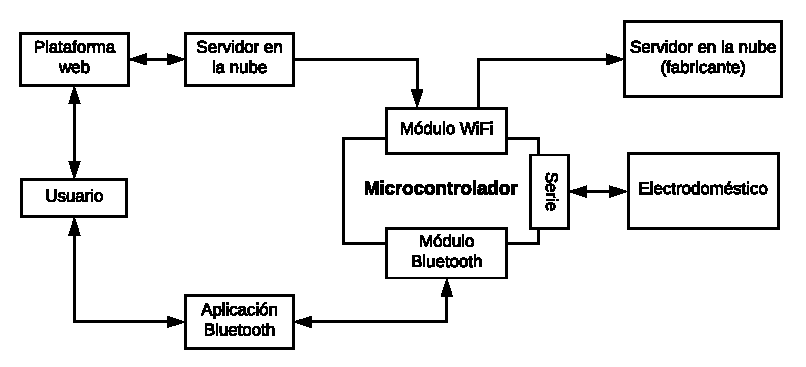
\includegraphics[width=\textwidth]{./Figures/simplified_diagram.pdf}
\caption{Diagrama general del sistema implementado.}
\label{fig:simplified_diagram}
\end{figure}

El principal componente del sistema es el microcontrolador, que se encarga de procesar los comandos recibidos y de gestionar todas las comunicaciones, para lo cual hace uso de sus interfaces de comunicación (módulos WiFi, Bluetooth y serie).

Para ilustrar el funcionamiento general del sistema, se presenta a continuación la serie de acciones que tiene lugar en un caso de uso típico del sistema, en el que el usuario desea que el electrodoméstico inicie una determinada operación (como por ejemplo, el ciclo de lavado en un lavarropas).

\begin{itemize}
	\item El usuario final le envía un comando al electrodoméstico, desde su computadora o celular.
	\begin{itemize}
		\item En caso de que el comando sea enviado por WiFi, la comunicación pasa a través de un servidor en la nube que recibe el comando del usuario y luego lo envía al microcontrolador.
		\item En caso de que el comando sea enviado por Bluetooth, la comunicación se realiza de manera directa con el microcontrolador.
	\end{itemize}
	\item El módulo correspondiente (módulo WiFi o Bluetooth, según sea el caso) recibe el comando y le informa al microcontrolador que hay un nuevo comando pendiente para procesar.
	\item El microcontrolador procesa el comando recibido y determina la acción a ejecutar.
	\item Si la acción a ejecutar lo requiere, el microcontrolador se comunica con la placa de control del electrodoméstico mediante una interfaz serie, a los fines de disparar en el mismo la operación deseada por el usuario.
	\item Dependiendo del tipo de acción, el electrodoméstico puede contestar con su información de estado, la cual es recibida por el microcontrolador y enviada de vuelta al usuario, a través de la misma interfaz desde la cual recibió el comando originalmente. Es decir, que si el usuario envió un comando por Bluetooth para consultar el estado del artefacto, el microcontrolador utiliza el módulo Bluetooth para devolverle la respuesta.
\end{itemize}

Cabe mencionar que, debido a limitaciones de hardware, las interfaces de comunicación WiFi y Bluetooth no pueden ser utilizadas en simultáneo. Por lo tanto, si se envían comandos por WiFi, el Bluetooth debe estar apagado, y viceversa al enviar comandos por Bluetooth. 

De manera independiente a las acciones disparadas a partir de un comando del usuario, el microcontrolador envía periódicamente al fabricante información acerca del estado del electrodoméstico. Este envío se lleva a cabo mediante la interfaz WiFi, que se comunica con un servidor en la nube solamente accesible por el fabricante, y que se encarga de almacenar la información para luego permitir su análisis y visualización. Gracias a esta información, el fabricante puede conocer y visualizar en todo momento el estado de sus electrodomésticos, ya sea de manera individual con todo el historial de uso de cada uno, o de forma general agrupando artefactos para obtener un panorama global del estado de sus dispositivos conectados.

Además, el módulo crea y mantiene activa en todo momento una red WiFi local de corto alcance en la que se encuentra corriendo un servidor web. El usuario puede conectarse a esta red y luego acceder desde cualquier navegador de Internet al servidor web, el cual permite configurar las credenciales de la red WiFi doméstica a la cual el módulo se conectará para recibir comandos y enviar información de uso al fabricante.

\section{Tecnologías inalámbricas}

En la actualidad, existen numerosas tecnologías inalámbricas que son aplicables a la Internet de las Cosas, muchas de las cuales incluso surgieron debido a la relevancia que este concepto fue tomando, como es el caso de NB-IoT \citep{nb_iot}, LoRa \citep{lora} y SigFox \citep{sigfox}. Muchas de estas tecnologías se caracterizan por permitir un bajo consumo de potencia y un largo alcance, a costa de una baja velocidad de transmisión, lo cual en muchas ocasiones es una relación de compromiso ideal para Internet de las Cosas.

A pesar del surgimiento de estas nuevas redes, las tecnologías tradicionales de conectividad inalámbrica, como el WiFi \citep{wifi} y el Bluetooth \citep{bluetooth}, siguen siendo adecuadas para muchas aplicaciones, especialmente aquellas que requieren una interacción directa con el usuario final. Esto se debe a que son tecnologías ampliamente soportadas por la gran mayoría de los dispositivos que posee una persona, como computadoras y celulares.

Un electrodoméstico conectado interactúa de manera directa con la persona que lo utiliza en el hogar, por lo tanto el WiFi y el Bluetooth son tecnologías sumamente adecuadas para un módulo destinado a tal fin.

La tecnología WiFi permite transmitir a grandes velocidades, pero con un alcance bajo y un consumo de energía mayor. Esto último impide que el WiFi sea utilizado en, por ejemplo, sensores que funcionan a batería ubicados en lugares remotos, pero no supone un problema para un electrodoméstico que se encuentra en el hogar, con fácil acceso a una fuente de alimentación y cerca de un punto de acceso al cual conectarse. 

Las especificaciones del WiFi definen una interfaz que se emplea para enviar y recibir señales entre un dispositivo inalámbrico (estación WiFi) y un punto de acceso. Si además se requiere tener acceso a Internet, es necesario conectarse también con un \emph{router} y un módem, el cual a su vez debe estar conectado a un proveedor de servicios de Internet (ISP, por sus siglas en inglés correspondientes a \emph{Internet Service Provider}). El módulo en el electrodoméstico actúa como una estación WiFi, es decir como un dispositivo que se conecta a la red doméstica de la casa y a través de ella obtiene una salida a Internet.

Por su parte, la tecnología Bluetooth pertenece a otro tipo de redes, denominadas Redes de Área Personal (PAN, por sus siglas en inglés) [ref]. Una conexión Bluetooth permite la comunicación directa entre dos dispositivos cercanos y su uso está sumamente masificado, ya que es fácil y económico integrarlo en muchos aparatos. Estas son características que lo convierten en una tecnología ideal para utilizar en un electrodoméstico conectado.

Su utilización en el ámbito de la Internet de las Cosas cobró verdadera importancia gracias al surgimiento del Bluetooth Low Energy (BLE) [ref], el cual fue diseñado específicamente para proporcionar un bajo consumo de energía. Esto permitió incrementar aún más la popularidad de la tecnología, extendiéndola hacia nuevos dispositivos como relojes o incluso zapatillas, lo cual fue acompañado con cada vez más modelos de computadores y celulares que también soporten la tecnología.


\section{Protocolos HTTP/S y MQTT}

Para que un dispositivo pueda conectarse a Internet, necesariamente debe recurrir al modelo TCP/IP \citep{tcp_ip_model}, cuyas diferentes capas pueden observarse en la figura \ref{fig:modelo_tcp_ip}.

\begin{figure}[h]
\centering
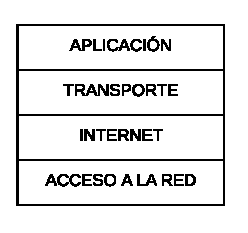
\includegraphics{./Figures/modelo_tcp_ip.pdf}
\caption{Capas del modelo TCP/IP.}
\label{fig:modelo_tcp_ip}
\end{figure}

El protocolo a nivel de capa de acceso a la red depende del hardware y del tipo de conectividad del dispositivo, y en el caso de este trabajo está constituida por la tecnología WiFi. Las capas de Internet y de transporte utilizan, en este trabajo, los protocolos que le dan el nombre al modelo, es decir IP (\emph{Internet Protocol}) y TCP (\emph{Transmission Control Protocol)}) respectivamente.

La capa de aplicación, ubicada en la parte superior del modelo, es la encargada de ofrecerle a las aplicaciones de usuario la posibilidad de comunicarse con otros dispositivos a través de los servicios brindados por las demás capas.

El protocolo de aplicación más conocido es el Protocolo de Transferencia de Hipertexto (HTTP por sus siglas en inglés, correspondientes a \emph{Hypertext Transfer Protocol}), el cual tiene una estructura cliente-servidor y permite realizar peticiones de datos y recursos \citep{http_protocol}. Este protocolo es la base de cualquier intercambio de datos en la web, y por lo tanto es utilizado en aplicaciones de Internet de las Cosas cuando se desea que el dispositivo conectado acceda directamente a diferentes páginas web.

Existe una variante denominada Protocolo Seguro de Transferencia de Hipertexto (HTTPS por sus siglas en inglés, correspondientes a \emph{Hypertext Transfer Protocol Secure}), que como su nombre lo indica, es una versión segura de HTTP en la que la transmisión está encriptada y el servidor autenticado \citep{https_protocol}. En toda aplicación, siempre se debe hacer lo posible para utilizar HTTPS y no simplemente HTTP, para garantizar la seguridad y la privacidad de los datos.

Además de los protocolos HTTP y HTTPS, existen otros protocolos para la capa de aplicación con características que los hacen ideales para la Internet de las Cosas, entre los que se destaca el protocolo MQTT (\emph{Message Queue Telemetry Transport}) \citep{mqtt_protocol}. Este protocolo se basa en un modelo de publicaciones y subscripciones, en el que un cliente publica mensajes en un tema o \emph{topic}, y todos aquellos nodos que se encuentran subscriptos a ese tema, reciben el mensaje publicado. MQTT es ideal para aplicaciones de IoT, debido principalmente a que requiere un muy bajo ancho de banda, tiene un menor consumo de potencia que otras alternativas, y además es sencillo y ligero de implementar.

Por todo lo enunciado anteriormente es que se decide que el módulo desarrollado soporte los 3 protocolos: HTTP, HTTPS y MQTT.

\section{Requerimientos}
\label{requerimientos}

A continuación se presentan los requerimientos en base a los cuales se desarrolló el presente trabajo, agrupados en cuatro categorías.
\begin{enumerate}
	\item Requerimientos generales del sistema.
	\begin{enumerate}
		\item El módulo debe ser capaz de llevar a cabo, mediante la recepción de comandos por
WiFi o Bluetooth, las mismas funciones que a través de la interfaz física del
electrodoméstico.
		\item El módulo debe ser capaz de enviar comandos por WiFi o Bluetooth, transmitiendo información de estado del electrodoméstico.
		\item Las acciones a ejecutar de acuerdo al comando recibido dependen de cada
aparato en particular, pero como mínimo se debe brindar la posibilidad de iniciar o
detener la acción del electrodoméstico y consultar su estado.
		\item El módulo debe enviar al fabricante información asociada al uso del
electrodoméstico, incluyendo el envío periódico del estado en el que se encuentra.
		\item El módulo debe ser capaz de crear su propia red local WiFi a los fines de
permitir configurar las credenciales de de la red WiFi a conectarse.
		\item El módulo debe ser capaz de enviar y recibir comandos por WiFi utilizando los
protocolos HTTP, HTTPS y MQTT.
	\end{enumerate}
	\item Requerimientos de hardware.
	\begin{enumerate}
		\item El módulo debe poder comunicarse utilizando el Estándar IEEE 802.11 b/g/n
(WiFi).
		\item El módulo debe poder comunicarse utilizando Bluetooth Low Energy (BLE).
		\item El módulo debe utilizar un único chip que integre el microprocesador y la conectividad WiFi/Bluetooth.
		\item El módulo debe contar como mínimo con interfaces de comunicación serie SPI (\emph{Serial Peripheral Interface}), I2C (\emph{Inter-Integrated Circuit}) y UART (\emph{Universal Asynchronous Receiver-Transmitter}), a los fines de poder adaptarse a los distintos tipos de electrodomésticos.
	\end{enumerate}
	\item Requerimientos de firmware.
	\begin{enumerate}
		\item El firmware del módulo debe ser programado en lenguaje C.
		\item Se deben realizar pruebas manuales para cada una de las funcionalidades del firmware del módulo.
	\end{enumerate}
	\item Requerimientos de gestión de proyectos.
	\begin{enumerate}
		\item Se debe utilizar YouTrack \citep{youtrack} como herramienta de \emph{issue tracking} y gestión de proyectos.
		\item Se debe usar Git como sistema de control de versiones.
	\end{enumerate}
\end{enumerate}

Cabe mencionar en este punto que originalmente se había planteado la integración del módulo a un electrodoméstico real, lo que implicaba también el diseño y fabricación de un PCB que se adapte al mismo. Sin embargo, debido a las dificultades para acceder a un electrodoméstico sobre el cual probar el módulo, sumado a la necesidad de acelerar los tiempos de desarrollo, se decidió reemplazar dicho electrodoméstico por otro microcontrolador que emule su comportamiento.


\section{Planificación}

Para mostrar la planificación del trabajo, se recurre a un diagrama \emph{Activity On Node} (figuras \ref{fig:activity_on_node_1}, \ref{fig:activity_on_node_2} y \ref{fig:activity_on_node_3}), en el cual cada caja o nodo representa una actividad, y las conexiones entre ellas representan una dependencia temporal en la que una debe terminarse antes que la siguiente. Además se muestra el tiempo en horas que demoraría cada una de las tareas.

\begin{figure}[h]
\centering
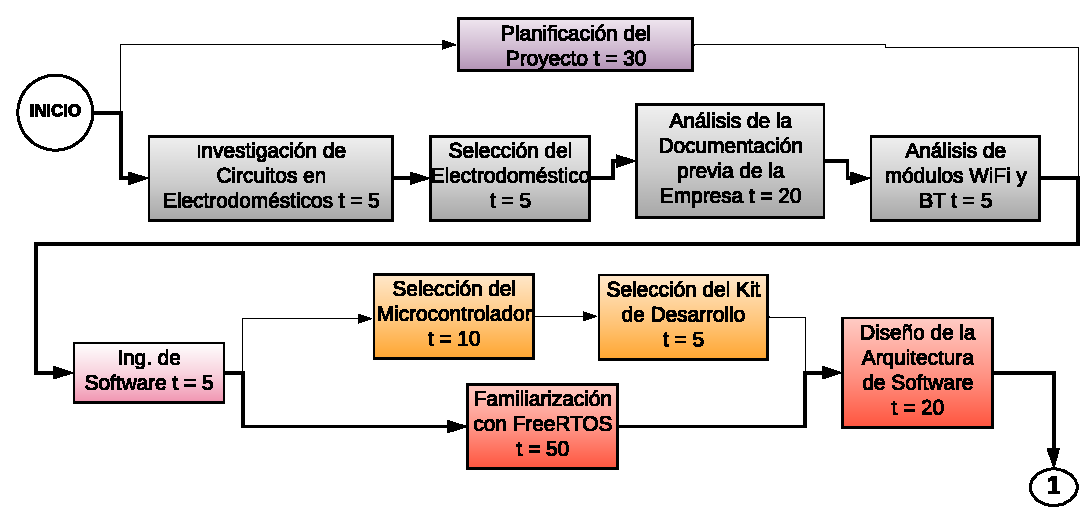
\includegraphics[width=\textwidth]{./Figures/activity_on_node_1.pdf}
\caption{Diagrama Activity On Node Parte 1.}
\label{fig:activity_on_node_1}
\end{figure}

Se puede observar que la primera etapa consiste en análisis e investigación, además de la planificación del trabajo propiamente dicha. Luego sigue una etapa de diseño de firmware y familiarización con las herramientas a utilizar, sin empezar aún con la implementación.

\begin{figure}[h]
\centering
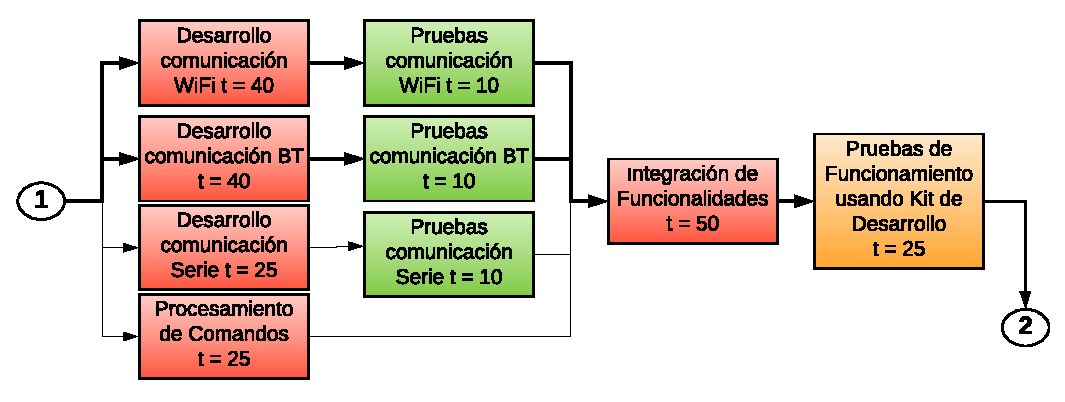
\includegraphics[width=\textwidth]{./Figures/activity_on_node_2.pdf}
\caption{Diagrama Activity On Node Parte 2.}
\label{fig:activity_on_node_2}
\end{figure}

Una vez definido el diseño, se procede con el desarrollo de las diferentes funcionalidades de firmware y sus respectivas pruebas. Si bien en el diagrama (figura \ref{fig:activity_on_node_2}) el desarrollo de estas tareas se muestra en paralelo, ya que son relativamente independientes y por lo tanto podrían ejecutarse en simultáneo, al ser desarrollado por una única persona, las tareas se debieron desarrollar en serie.

Luego se integran todas las funcionalidades implementadas y se realizan pruebas generales del sistema, para posteriormente configurar las plataformas utilizadas para enviar y recibir información por WiFi y Bluetooth.

\begin{figure}[h]
\centering
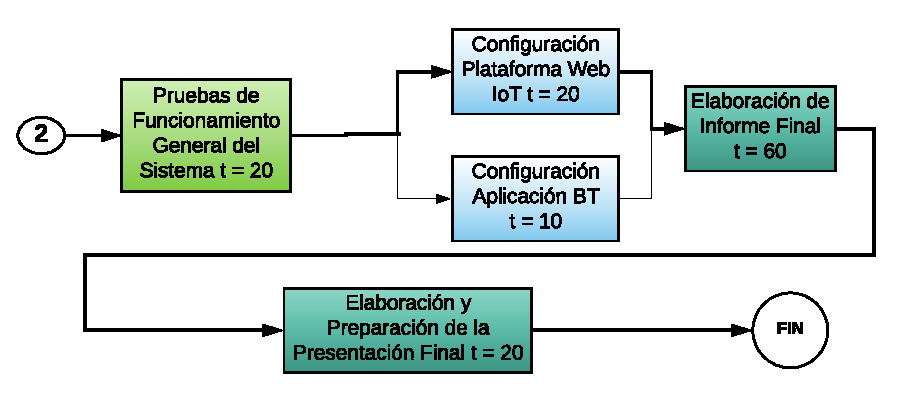
\includegraphics[width=\textwidth]{./Figures/activity_on_node_3.pdf}
\caption{Diagrama Activity On Node Parte 3.}
\label{fig:activity_on_node_3}
\end{figure}

Finalmente se contempla también el tiempo necesario para las actividades asociadas a la presentación del trabajo final.


%\begin{figure}[h]
%\centering
%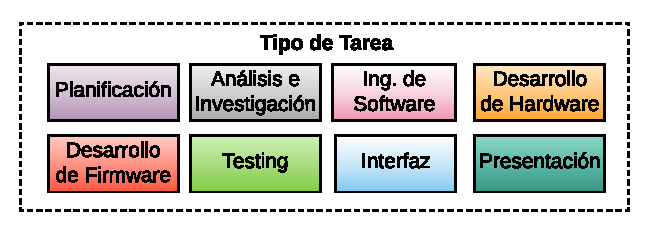
\includegraphics[width=\textwidth]{./Figures/activity_on_node_4.pdf}
%\caption{Referencias del diagrama Activity On Node.}
%\label{fig:activity_on_node_4}
%\end{figure}


 
	\chapter{Diseño e Implementación} % Main chapter title

\label{Chapter3} % Change X to a consecutive number; for referencing this chapter elsewhere, use \ref{ChapterX}

\definecolor{mygreen}{rgb}{0,0.6,0}
\definecolor{mygray}{rgb}{0.5,0.5,0.5}
\definecolor{mymauve}{rgb}{0.58,0,0.82}

%%%%%%%%%%%%%%%%%%%%%%%%%%%%%%%%%%%%%%%%%%%%%%%%%%%%%%%%%%%%%%%%%%%%%%%%%%%%%
% parámetros para configurar el formato del código en los entornos lstlisting
%%%%%%%%%%%%%%%%%%%%%%%%%%%%%%%%%%%%%%%%%%%%%%%%%%%%%%%%%%%%%%%%%%%%%%%%%%%%%
\lstset{ %
  backgroundcolor=\color{white},   % choose the background color; you must add \usepackage{color} or \usepackage{xcolor}
  basicstyle=\footnotesize,        % the size of the fonts that are used for the code
  breakatwhitespace=false,         % sets if automatic breaks should only happen at whitespace
  breaklines=true,                 % sets automatic line breaking
  captionpos=b,                    % sets the caption-position to bottom
  commentstyle=\color{mygreen},    % comment style
  deletekeywords={...},            % if you want to delete keywords from the given language
  %escapeinside={\%*}{*)},          % if you want to add LaTeX within your code
  %extendedchars=true,              % lets you use non-ASCII characters; for 8-bits encodings only, does not work with UTF-8
  %frame=single,	                % adds a frame around the code
  keepspaces=true,                 % keeps spaces in text, useful for keeping indentation of code (possibly needs columns=flexible)
  keywordstyle=\color{blue},       % keyword style
  language=[ANSI]C,                % the language of the code
  %otherkeywords={*,...},           % if you want to add more keywords to the set
  numbers=left,                    % where to put the line-numbers; possible values are (none, left, right)
  numbersep=5pt,                   % how far the line-numbers are from the code
  numberstyle=\tiny\color{mygray}, % the style that is used for the line-numbers
  rulecolor=\color{black},         % if not set, the frame-color may be changed on line-breaks within not-black text (e.g. comments (green here))
  showspaces=false,                % show spaces everywhere adding particular underscores; it overrides 'showstringspaces'
  showstringspaces=false,          % underline spaces within strings only
  showtabs=false,                  % show tabs within strings adding particular underscores
  stepnumber=1,                    % the step between two line-numbers. If it's 1, each line will be numbered
  stringstyle=\color{mymauve},     % string literal style
  tabsize=2,	                   % sets default tabsize to 2 spaces
  title=\lstname,                  % show the filename of files included with \lstinputlisting; also try caption instead of title
  morecomment=[s]{/*}{*/}
}


%----------------------------------------------------------------------------------------
%	SECTION 1
%----------------------------------------------------------------------------------------
\section{Análisis del software}
 
La idea de esta sección es resaltar los problemas encontrados, los criterios utilizados y la justificación de las decisiones que se hayan tomado.

Se puede agregar código o pseudocódigo dentro de un entorno lstlisting con el siguiente código:

\begin{verbatim}
\begin{lstlisting}[caption= "un epígrafe descriptivo"]
	las líneas de código irían aquí...
\end{lstlisting}
\end{verbatim}

A modo de ejemplo:

\begin{lstlisting}[label=cod:vControl,caption=Pseudocódigo del lazo principal de control.]  % Start your code-block

#define MAX_SENSOR_NUMBER 3
#define MAX_ALARM_NUMBER  6
#define MAX_ACTUATOR_NUMBER 6

uint32_t sensorValue[MAX_SENSOR_NUMBER];		
FunctionalState alarmControl[MAX_ALARM_NUMBER];	//ENABLE or DISABLE
state_t alarmState[MAX_ALARM_NUMBER];						//ON or OFF
state_t actuatorState[MAX_ACTUATOR_NUMBER];			//ON or OFF

void vControl() {

	initGlobalVariables();
	
	period = 500 ms;
		
	while(1) {

		ticks = xTaskGetTickCount();
		
		updateSensors();
		
		updateAlarms();
		
		controlActuators();
		
		vTaskDelayUntil(&ticks, period);
	}
}
\end{lstlisting}




	% Chapter Template

\chapter{Ensayos y Resultados} % Main chapter title
\label{Chapter4}

En este capítulo se presentan las pruebas realizadas para validar el correcto funcionamiento del sistema implementado. Se incluyen pruebas funcionales de cada bloque en particular y también de todo el sistema integrado.

\section{Pruebas funcionales}

A medida que se desarrollaron los diferentes módulos del firmware del sistema, se llevaron a cabo las correspondientes pruebas en cada uno de ellos, para validar que funcionaban de la manera esperada antes de ser integrados con otras partes del sistema. Todas las pruebas fueron realizadas manualmente.

Los bloques a probar se pueden dividir en tres: la comunicación por WiFi, la comunicación utilizando BLE y la comunicación con el electrodoméstico.

\subsection{Comunicación WiFi}

La comunicación por WiFi es la parte del sistema más compleja y la que por lo tanto requiere pruebas más exhaustivas de sus diferentes funcionalidades.

Independientemente de la aplicación que se le vaya a dar, el primer paso es lograr conectarse exitosamente a una red WiFi. Esta fue la primera prueba realizada, configurando a mano las credenciales de la red inalámbrica y verificando por consola que se conecte correctamente, como se puede ver en la figura \ref{fig:output_wifi_connection}. En ella, se ve que se inició la conexión y luego se registró el evento en el que el microcontrolador obtuvo una dirección IP y por lo tanto se conectó con éxito.

\begin{figure}[h]
\centering
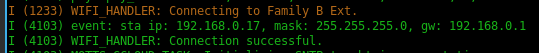
\includegraphics[width=\textwidth]{./Figures/output_wifi_connection.png}
\caption{Salida por consola del microcontrolador al conectarse a una red WiFi.}
\label{fig:output_wifi_connection}
\end{figure}

Una vez llegado a este punto, es posible continuar con las pruebas asociadas a la comunicación con el usuario del electrodoméstico, mediante una interfaz de usuario, y con el fabricante, enviando información hacia Google Cloud.

\subsubsection{Comunicación con el usuario}

Si bien en los alcances del trabajo se especificó que no se incluía el desarrollo de una interfaz web desde la cual el usuario pudiese interactuar con el electrodoméstico, de todos modos se requiere contar con algún mecanismo para enviar comandos desde Internet para verificar el correcto funcionamiento. Por ello es que se recurrió a diferentes plataformas web IoT configurables ya existentes.

Para las pruebas de envío y recepción mediante los protocolos HTTP y HTTPS, se utilizó ThingSpeak \citep{thingspeak}. Esta plataforma permite recibir información desde el microcontrolador, almacenarla y graficarla. Además permite enviar comandos desde la página hacia el microcontrolador. Si bien ThingSpeak ofrece una librería para interactuar con la plataforma, en este caso se utilizaron directamente las direcciones indicadas en su documentación para enviar HTTP \emph{requests} desde las tareas de transmisión y recepción WiFi que se ejecutan en el microcontrolador. De esta forma por un lado se enviaron comandos desde ThingSpeak y se observó por consola que el microcontrolador los recibía correctamente. Por otro lado se enviaron datos periódicamente hacia ThingSpeak y se los graficó, verificando que tienen los valores esperados.

Para demostrar la versatilidad del módulo desarrollado, se decidió utilizar una plataforma IoT diferente para probar la comunicación utilizando MQTT. Por eso se utilizó Adafruit IO \citep{adafruit}, plataforma que permite crear tableros o \emph{dashboards} personalizados para comunicarse con sistemas embebidos. La figura \ref{fig:adafruit_dashboard} muestra la interfaz desarrollada, en la que se puede ver que se tienen diferentes botones para enviar comandos determinados, un historial de comandos enviados, un cuadro mostrando el estado del electrodoméstico (\emph{slave}) y un cuadro con el último comando enviado.

\begin{figure}[h]
\centering
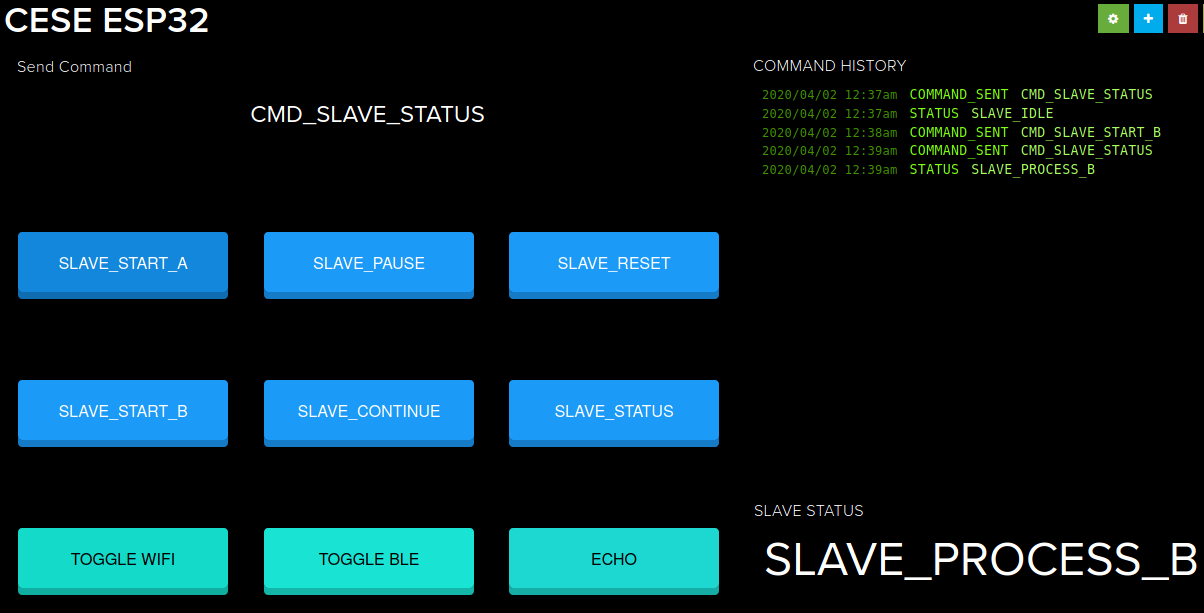
\includegraphics[width=\textwidth]{./Figures/adafruit_dashboard.png}
\caption{Interfaz de usuario creada en Adafruit IO.}
\label{fig:adafruit_dashboard}
\end{figure}

En el historial de comandos se puede observar que se envió un comando para conocer el estado del electrodoméstico (CMD\_SLAVE\_STATUS) y se recibió de vuelta el estado actual (SLAVE\_IDLE, es decir inactivo sin ejecutar ninguna acción). Luego se envió un comando para iniciar un proceso en el electrodoméstico (CMD\_SLAVE\_PROCESS\_B), y al preguntar nuevamente por el estado, se obtuvo que se encontraba ejecutando la acción iniciada con el comando anterior.

Desde el punto de vista del firmware, en la figura \ref{fig:output_mqtt_connection} se observa cómo van ocurriendo los diferentes eventos asociados a MQTT (descriptos en la sección \ref{sec:wifi_com}). 

\begin{figure}[h]
\centering
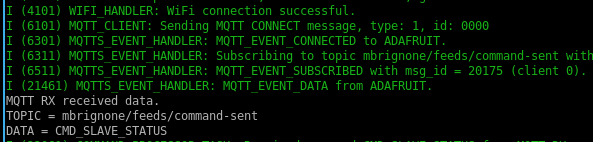
\includegraphics[width=\textwidth]{./Figures/output_mqtt_connection.png}
\caption{Eventos disparados en el microcontrolador por la comunicación utilizando MQTT.}
\label{fig:output_mqtt_connection}
\end{figure}

Primero se espera a que el \emph{driver} WiFi indique que la conexión ya está habilitada, y luego se envía la orden de conectarse al \emph{broker} MQTT, disparándose a continuación el evento MQTT\_EVENT\_CONNECTED, el cual indica que la conexión al \emph{broker} fue exitosa. 

Para detectar los comandos enviados por el usuario, el cliente se suscribe al \emph{topic} correspondiente, lo cual dispara el evento MQTT\_EVENT\_SUBSCRIBED.

Finalmente, se dispara el evento MQTT\_EVENT\_DATA indicando que hay un dato nuevo en el \emph{topic} al cual el microcontrolador se encuentra suscrito, y se puede ver que el dato recibido se corresponde al comando enviado desde Adafruit.

\subsubsection{Comunicación con el fabricante}

La comunicación con el fabricante consiste en el envío de datos desde el microcontrolador hacia Google Cloud utilizando el protocolo MQTT. Para ello primero el dispositivo debe conectarse al \emph{broker} de Google Cloud y autenticarse mediante un JSON Web Token, tal como se explicó en la sección \ref{sec:google_cloud}. Este proceso se puede observar en la figura \ref{fig:output_gcloud_connection}, donde se aprecia cómo se generó el JWT, para lo cual se obtuvo el tiempo actual mediante el protocolo SNTP, y luego se conectó a Google Cloud.

\begin{figure}[h]
\centering
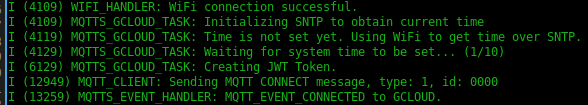
\includegraphics[width=\textwidth]{./Figures/output_gcloud_connection.png}
\caption{Conexión del microcontrolador a Google Cloud por MQTT.}
\label{fig:output_gcloud_connection}
\end{figure}

Una vez conectado al \emph{broker}, se enviaron algunos mensajes y luego se revisó el registro de eventos (\emph{logs}) de Google Cloud para verificar que la comunicación fue exitosa. Esto se ilustra en la figura \ref{fig:gcloud_log}, en la que se ve que primero se produce la conexión de un dispositivo, luego la publicación de dos mensajes y finalmente la desconexión del dispositivo. Cabe mencionar que en el registro se cuenta con mucha más información que la mostrada en la figura \ref{fig:gcloud_log}, pero se la omite por simplicidad.

\begin{figure}[h]
\centering
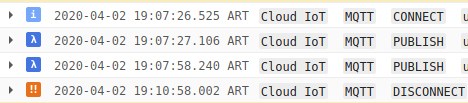
\includegraphics[width=\textwidth]{./Figures/gcloud_log.png}
\caption{Registro de eventos MQTT en Google Cloud.}
\label{fig:gcloud_log}
\end{figure}

\subsubsection{Servidor web}

\subsection{Comunicación BLE}

\subsection{Comunicación serie con electrodoméstico}

\section{Integración del sistema}

\subsection{Visualización de datos en Google Cloud Platform}
























 
	% Chapter Template

\chapter{Conclusiones} % Main chapter title

\label{Chapter5} % Change X to a consecutive number; for referencing this chapter elsewhere, use \ref{ChapterX}


%----------------------------------------------------------------------------------------

%----------------------------------------------------------------------------------------
%	SECTION 1
%----------------------------------------------------------------------------------------

\section{Conclusiones generales }

La idea de esta sección es resaltar cuáles son los principales aportes del trabajo realizado y cómo se podría continuar. Debe ser especialmente breve y concisa. Es buena idea usar un listado para enumerar los logros obtenidos.

Algunas preguntas que pueden servir para completar este capítulo:

\begin{itemize}
\item ¿Cuál es el grado de cumplimiento de los requerimientos?
\item ¿Cuán fielmente se puedo seguir la planificación original (cronograma incluido)?
\item ¿Se manifestó algunos de los riesgos identificados en la planificación? ¿Fue efectivo el plan de mitigación? ¿Se debió aplicar alguna otra acción no contemplada previamente?
\item Si se debieron hacer modificaciones a lo planificado ¿Cuáles fueron las causas y los efectos?
\item ¿Qué técnicas resultaron útiles para el desarrollo del proyecto y cuáles no tanto?
\end{itemize}


%----------------------------------------------------------------------------------------
%	SECTION 2
%----------------------------------------------------------------------------------------
\section{Próximos pasos}

Acá se indica cómo se podría continuar el trabajo más adelante.
 
\end{verbatim}

Los apéndices también deben escribirse en archivos .tex separados, que se deben ubicar dentro de la carpeta \emph{Appendices}. Los apéndices vienen comentados por defecto con el caracter \code{\%} y para incluirlos simplemente se debe eliminar dicho caracter.

Finalmente, se encuentra el código para incluir la bibliografía en el documento final.  Este código tampoco debe modificarse. La metodología para trabajar las referencias bibliográficas se desarrolla en la sección \ref{sec:biblio}.
%----------------------------------------------------------------------------------------

\section{Bibliografía}
\label{sec:biblio}

Las opciones de formato de la bibliografía se controlan a través del paquete de latex \option{biblatex} que se incluye en la memoria en el archivo memoria.tex.  Estas opciones determinan cómo se generan las citas bibliográficas en el cuerpo del documento y cómo se genera la biblografía al final de la memoria.

En el preámbulo se puede encontrar el código que incluye el paquete biblatex, que no requiere ninguna modificación del usuario de la plantilla, y que contiene las siguientes opciones:

\begin{lstlisting}
\usepackage[backend=bibtex,
	natbib=true, 
	style=numeric, 
	sorting=none]
{biblatex}
\end{lstlisting}

En el archivo \file{reference.bib} se encuentran las referencias bibliográficas que se pueden citar en el documento.  Para incorporar una nueva cita al documento lo primero es agregarla en este archivo con todos los campos necesario.  Todas las entradas bibliográficas comienzan con $@$ y una palabra que define el formato de la entrada.  Para cada formato existen campos obligatorios que deben completarse. No importa el orden en que las entradas estén definidas en el archivo .bib.  Tampoco es importante el orden en que estén definidos los campos de una entrada bibliográfica. A continuación se muestran algunos ejemplos:

\begin{lstlisting}
@ARTICLE{ARTICLE:1,
    AUTHOR="John Doe",
    TITLE="Title",
    JOURNAL="Journal",
    YEAR="2017",
}
\end{lstlisting}


\begin{lstlisting}
@BOOK{BOOK:1,
    AUTHOR="John Doe",
    TITLE="The Book without Title",
    PUBLISHER="Dummy Publisher",
    YEAR="2100",
}
\end{lstlisting}


\begin{lstlisting}
@INBOOK{BOOK:2,
    AUTHOR="John Doe",
    TITLE="The Book without Title",
    PUBLISHER="Dummy Publisher",
    YEAR="2100",
    PAGES="100-200",
}
\end{lstlisting}


\begin{lstlisting}
@MISC{WEBSITE:1,
    HOWPUBLISHED = "\url{http://example.com}",
    AUTHOR = "Intel",
    TITLE = "Example Website",
    MONTH = "12",
    YEAR = "1988",
    URLDATE = {2012-11-26}
}
\end{lstlisting}

Se debe notar que los nombres \emph{ARTICLE:1}, \emph{BOOK:1}, \emph{BOOK:2} y \emph{WEBSITE:1} son nombres de fantasía que le sirve al autor del documento para indentificar la entrada. En este sentido, se podrían reemplazar por cualquier otro nombre.  Tampoco es necesario poner : seguido de un número, en los ejemplos sólo se incluye como un posible estilo para identificar las entradas.

La entradas se citan en el documento con el comando: 

\begin{verbatim}
\citep{nombre_de_la_entrada}
\end{verbatim}

Y cuando se usan, se muestran así: \citep{ARTICLE:1}, \citep{BOOK:1}, \citep{BOOK:2}, \citep{WEBSITE:1}.  Notar cómo se conforma la sección Bibliografía al final del documento. 